\subsection{Communications serveur-drone}\label{impl}
Pour établir les communications entre le serveur et le drone, nous nous sommes dirigés vers les API permettant de piloter notre drone à distance. Le drone étant un \textit{Parrot BEBOP 2} nous nous sommes intéressé à la SDK ARSDK fourni par le constructeur. Nous avons rencontré des difficultés pour mettre en place l'environnement de développement : la méthode de compilation n'était pas usuelle et la gestion des dépendances s'est avérée compliquée. À première vue, il semblait y avoir une version compatible avec Java, le langage que nous avons utilisé pour le serveur et pour le client via la SDK \android{}.

Cependant cette version de la SDK n'était destinée qu'à développer des applications mobiles \android{}, nous avons du considérer l'API C à la place.

Pour comprendre comment utiliser les primitives disponibles, nous avons étudié l'exemple fourni : la documentation étant trop pauvre pour suffire. Cet exemple permet de piloter un drone à distance à l'aide d'un ordinateur connecté en Wi-Fi et d'avoir un retour vidéo du drone. Comme la communication entre l'appareil manipulant le drone et celui-ci est en Wi-Fi, le serveur de jeu, et, par extension, les clients \android{} devront être connectés au réseau sans fil du drone pour la communication.

\paragraph{}
Nous avons commencé par faire de courts programmes C permettant de nous connecter au drone et de le faire décoller puis avancer en ligne droite, reculer et répéter ces opérations plusieurs fois avant de se poser pour terminer. La principale difficulté pour cette partie de tests fut de trouver des moments de libre à la fac où le drone était disponible, cela nous a considérable ralenti dans notre développement.

Nous avons ensuite décidé d'appeler à la place des routines C depuis Java en créant un programme supplémentaire chargé de piloter le drone et le connecter au serveur de jeu par le biais d'une \textit{socket} TCP.
Par mesure de sécurité, nous avons décidé de mettre en place un mode de pilotage manuel sur lequel on peut basculer à tout moment.

\paragraph{}
Il nous reste à implémenter le déplacement du drone en fonction du score des joueurs et de l'avancement du niveau. L'idée en théorie serait, par exemple pour deux joueurs, de positionner le drone au centre d'un segment passant par les deux joueurs, et définir la distance par rapport au centre du segment avec l'avancement du niveau dans la direction du joueur gagnant.
Une autre possibilité serait de décider d'une fréquence pour déplacer le drone dans la direction du joueur qui mène la partie.

\begin{figure}[ht]
\begin{center}
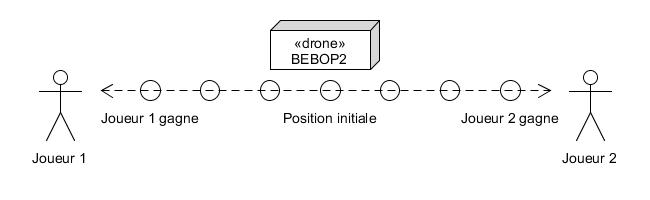
\includegraphics[scale=0.5]{images/partie.jpg}
\caption{Schéma du déroulement d'une partie}
\end{center}
\end{figure}